%% Modello computazionale
% descrivere il problema della computazione distribuita nel nostro contesto

% io parto da questa architettura che funziona così...
% ho un'architettura di riferimento con una macchina/mainframe centralizzata che definisce e distribuisce il
% carico di lavoro ed il calcolo; ho tanti client trasparenti/coerenti con i browser e poi gli utenti
% Immagine di come funziona


%Architettura:
% Modello statico->
% DEfinizione di cos'è uno User
% DEfinizione di cos'è un uTask
% DEfinizione di cos'è un Task generico

% Modello astratto->
%% TASK: dal punto di vista astratto è la definizione di un'operazione data driven
% su un modello di dati in ingresso e un modello di uscita, in cui posso caratterizzare
% cosa ci sta im mezzo in modo preciso con associato un codice di esecuzione.
%% Utente: è una persona con una macchina con certe caratteistiche e certe skill lui
%% uTask: istanziazione di un task con un particolare codice su una particolare macchina su dei dati

% TODO nell'immagine metto anche un dispositivo mobile e un utente con 2 device
\begin{figure}[htb]
	\centering
	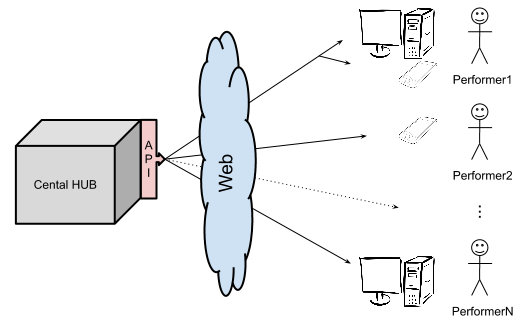
\includegraphics[width=0.75\columnwidth]{Architecture.png}
	\caption{Reference architecture.}
	\label{fig:architecture}
\end{figure}
The system use as a reference architecture the one depicted in \autoref{fig:architecture}.
Here we have a centralized hub that \emph{defines} and \emph{distribute} the workload,
a pletora of clients with their browsers and the users. The clients of this model
are all coherent and transparent to the execution of the code, wich is distributed
to the end-user according to the platform they are using.
As you can see the structure is almost the same as any other task distribution
platform, the strenghts of this system are in the characterization of the actors
in the system.

The reference model in \autoref{fig:architecture} has been customized to meet our
needs of flexibility and pluggability, so we introduced a \emph{configurator} and
a \emph{execution layer} in the central hub. These are the components that allow
our system to cover all the dimension presented in \autoref{tab:matrix}.

The \textbf{configurator} is in charge of defining and configuring a task in the
system, allowing the \emph{requester} to add hooks to exeternal resource in order
to manage the assignment cycle and the planning strategy.

The \textbf{execution layer} provides useful API for managing the \utask{} and
communicate with the \emph{configurator}.

\begin{figure}[tb]
	\centering
	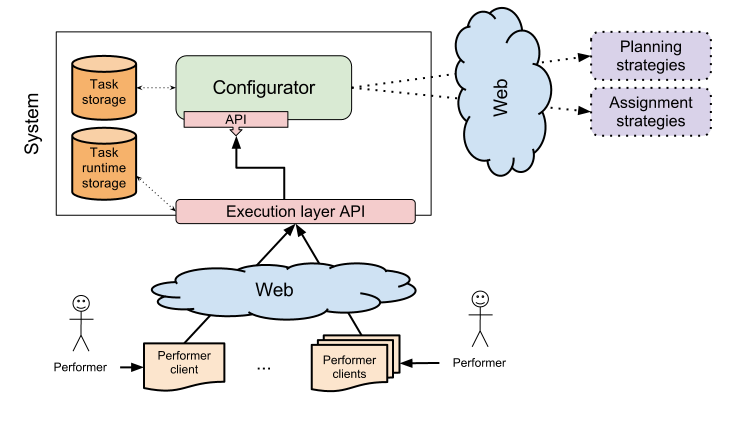
\includegraphics[width=\columnwidth]{Architecture2.png}
	\caption{Specialized architecture.}
	\label{fig:architecture2}
\end{figure}




% Subsection description

\subsection{Configurator}
The \textbf{Configurator} is the component in charge of the task lifecycle
management. The principal functionalities offered by the \textbf{Configurator}
are:
\begin{itemize}
	\item Allow the \textbf{creation} of a Task, also at abstract level, using
	either the API or the built-in UI.

	\item Allow a \emph{Performer} to \textbf{execute} the Task using a standard
	non configurable UI, provided as-is for each Task type.

	\item Allow to \textbf{request information} about a Task, the information
	that can be requested includes:
	\begin{itemize}
		\item Retrieve the list of \utask{} associated with a given Task

		\item Post the result of the execution of a given \utask{}

		\item Notify about the completion of a Task or \utask{}
	\end{itemize}
\end{itemize}

Alongside these main functionalities it offer a \emph{Requester} the ability to
monitor the state of a Task and/or a \utask{}.




\subsection{Execution layer}
This component is in charge of managing the \utask{} implementation for each Task
or for each \utask{}. The implementations have a fallback behaviour so, if a
custom \utask{} implementation is not present then the system search for a
custom Task implementation, if this is missing then the built-in implementation
is used. On top of this fallback system the component offer the possibility to
create code for a target platform.

The \textbf{Execution layer} offer the following funcionalities:
\begin{itemize}
	\item Allow a \emph{Requester} to configure the implementations associated to
	a Task and/or a \utask{}. The implementations are configured specifing the
	target platform (mobile, desktop, tablet, ...) and the executable resources
	used by the implementation (i.e. HTML, CSS and JS files). Wich implementation
	to use is configured later in the \emph{Planning} step.

	\item Create a layer of abstraction between the implementation and the
	Configurator, creating a sandboxed environment where the implementation can
	run and communicate with the Configurator.

	\item Allow the \emph{Performer} to execute a specific \utask{} implementation.
\end{itemize}






\subsection{Task storage \& task runtime storage}
These are the storage areas where we put all the data associated with the Task.
We used two separated storage area in order to keep the runtime configuration
separated from the abstract configuration data of the Task.

The task runtime storage contains all the ad-hoc code written by the \emph{Requester}
for each platform.
% Codice che può diventare generico
\textbf{This code can be reused by the other \emph{Requester} to execute the same
task (for example image tagging).}





\subsection{Performer \& Performer client}
The \emph{Performer client} represents the platform (like desktop or mobile) on
wich a \emph{Performer} executes the Task implementation. The \emph{Performer
client} make use of the \emph{Execution layer API} to retrieve the correct
implementation, communicate the status during the exection of a \utask{} and
post the result of the execution. The \emph{Performer} is the actual user that
is using the \emph{client}.



\subsection{Planning strategies}
Any third-part component in charge of the creation and management of the \utask{}
associated with a Task. During the Task configuration step the \emph{Requester}
decide when this external component need to be called. The \emph{Planning
strategy} can be called only once, for example during the task creation, or
ca behave like an handler to the \utask{} ended event, in this case the
\emph{stategy} is able to decide wheter is necessary to spawn other \utask{}
execution to fullfill the requirements.



\subsection{Assignment strategies}
Any third-part component used to associate \utask{} to Performers. The binding
can leverage on some skill of the Performer, for example a stategy can be:
associate this set of \utask{} to Performers skilled German translation, and
all the other to any Performer. As for the \emph{Planning strategies} this
component can be invoked only once or in response to some events (like \utask{}
ended or created).